% Options for packages loaded elsewhere
\PassOptionsToPackage{unicode}{hyperref}
\PassOptionsToPackage{hyphens}{url}
\PassOptionsToPackage{dvipsnames,svgnames,x11names}{xcolor}
\documentclass[
]{report}
\usepackage{xcolor}
\usepackage{graphicx}
\usepackage{tikz}
\usetikzlibrary{arrows.meta,positioning,shapes.geometric,fit}
\usepackage[margin=1in]{geometry}
\usepackage{amsmath,amssymb}
\setcounter{secnumdepth}{-\maxdimen} % remove section numbering
\usepackage{iftex}
\ifPDFTeX
  \usepackage[T1]{fontenc}
  \usepackage[utf8]{inputenc}
  \usepackage{textcomp} % provide euro and other symbols
\else % if luatex or xetex
  \usepackage{unicode-math} % this also loads fontspec
  \defaultfontfeatures{Scale=MatchLowercase}
  \defaultfontfeatures[\rmfamily]{Ligatures=TeX,Scale=1}
\fi
\usepackage{lmodern}
\ifPDFTeX\else
  % xetex/luatex font selection
\fi
% Use upquote if available, for straight quotes in verbatim environments
\IfFileExists{upquote.sty}{\usepackage{upquote}}{}
\IfFileExists{microtype.sty}{% use microtype if available
  \usepackage[]{microtype}
  \UseMicrotypeSet[protrusion]{basicmath} % disable protrusion for tt fonts
}{}
\makeatletter
\@ifundefined{KOMAClassName}{% if non-KOMA class
  \IfFileExists{parskip.sty}{%
    \usepackage{parskip}
  }{% else
    \setlength{\parindent}{0pt}
    \setlength{\parskip}{6pt plus 2pt minus 1pt}}
}{% if KOMA class
  \KOMAoptions{parskip=half}}
\makeatother
\usepackage{color}
\usepackage{fancyvrb}
\newcommand{\VerbBar}{|}
\newcommand{\VERB}{\Verb[commandchars=\\\{\}]}
\DefineVerbatimEnvironment{Highlighting}{Verbatim}{commandchars=\\\{\}}
% Add ',fontsize=\small' for more characters per line
\newenvironment{Shaded}{}{}
\newcommand{\AlertTok}[1]{\textcolor[rgb]{1.00,0.00,0.00}{\textbf{#1}}}
\newcommand{\AnnotationTok}[1]{\textcolor[rgb]{0.38,0.63,0.69}{\textbf{\textit{#1}}}}
\newcommand{\AttributeTok}[1]{\textcolor[rgb]{0.49,0.56,0.16}{#1}}
\newcommand{\BaseNTok}[1]{\textcolor[rgb]{0.25,0.63,0.44}{#1}}
\newcommand{\BuiltInTok}[1]{\textcolor[rgb]{0.00,0.50,0.00}{#1}}
\newcommand{\CharTok}[1]{\textcolor[rgb]{0.25,0.44,0.63}{#1}}
\newcommand{\CommentTok}[1]{\textcolor[rgb]{0.38,0.63,0.69}{\textit{#1}}}
\newcommand{\CommentVarTok}[1]{\textcolor[rgb]{0.38,0.63,0.69}{\textbf{\textit{#1}}}}
\newcommand{\ConstantTok}[1]{\textcolor[rgb]{0.53,0.00,0.00}{#1}}
\newcommand{\ControlFlowTok}[1]{\textcolor[rgb]{0.00,0.44,0.13}{\textbf{#1}}}
\newcommand{\DataTypeTok}[1]{\textcolor[rgb]{0.56,0.13,0.00}{#1}}
\newcommand{\DecValTok}[1]{\textcolor[rgb]{0.25,0.63,0.44}{#1}}
\newcommand{\DocumentationTok}[1]{\textcolor[rgb]{0.73,0.13,0.13}{\textit{#1}}}
\newcommand{\ErrorTok}[1]{\textcolor[rgb]{1.00,0.00,0.00}{\textbf{#1}}}
\newcommand{\ExtensionTok}[1]{#1}
\newcommand{\FloatTok}[1]{\textcolor[rgb]{0.25,0.63,0.44}{#1}}
\newcommand{\FunctionTok}[1]{\textcolor[rgb]{0.02,0.16,0.49}{#1}}
\newcommand{\ImportTok}[1]{\textcolor[rgb]{0.00,0.50,0.00}{\textbf{#1}}}
\newcommand{\InformationTok}[1]{\textcolor[rgb]{0.38,0.63,0.69}{\textbf{\textit{#1}}}}
\newcommand{\KeywordTok}[1]{\textcolor[rgb]{0.00,0.44,0.13}{\textbf{#1}}}
\newcommand{\NormalTok}[1]{#1}
\newcommand{\OperatorTok}[1]{\textcolor[rgb]{0.40,0.40,0.40}{#1}}
\newcommand{\OtherTok}[1]{\textcolor[rgb]{0.00,0.44,0.13}{#1}}
\newcommand{\PreprocessorTok}[1]{\textcolor[rgb]{0.74,0.48,0.00}{#1}}
\newcommand{\RegionMarkerTok}[1]{#1}
\newcommand{\SpecialCharTok}[1]{\textcolor[rgb]{0.25,0.44,0.63}{#1}}
\newcommand{\SpecialStringTok}[1]{\textcolor[rgb]{0.73,0.40,0.53}{#1}}
\newcommand{\StringTok}[1]{\textcolor[rgb]{0.25,0.44,0.63}{#1}}
\newcommand{\VariableTok}[1]{\textcolor[rgb]{0.10,0.09,0.49}{#1}}
\newcommand{\VerbatimStringTok}[1]{\textcolor[rgb]{0.25,0.44,0.63}{#1}}
\newcommand{\WarningTok}[1]{\textcolor[rgb]{0.38,0.63,0.69}{\textbf{\textit{#1}}}}
\usepackage{longtable,booktabs,array}
\usepackage{calc} % for calculating minipage widths
% Correct order of tables after \paragraph or \subparagraph
\usepackage{etoolbox}
\makeatletter
\patchcmd\longtable{\par}{\if@noskipsec\mbox{}\fi\par}{}{}
\makeatother
% Allow footnotes in longtable head/foot
\IfFileExists{footnotehyper.sty}{\usepackage{footnotehyper}}{\usepackage{footnote}}
\makesavenoteenv{longtable}
\setlength{\emergencystretch}{3em} % prevent overfull lines
\providecommand{\tightlist}{%
  \setlength{\itemsep}{0pt}\setlength{\parskip}{0pt}}
\usepackage{bookmark}
\IfFileExists{xurl.sty}{\usepackage{xurl}}{} % add URL line breaks if available
\urlstyle{same}
\hypersetup{
  colorlinks=true,
  linkcolor={blue},
  filecolor={Maroon},
  citecolor={Blue},
  urlcolor={blue},
  pdfcreator={LaTeX via pandoc}}

\author{}
\date{}

\begin{document}

\begin{titlepage}
  \centering
  \vspace*{1.2cm}
  {\Large Seneca Polytechnic\par}
  \vspace{0.5cm}
  {\large SED800 - Software Engineering Capstone\par}
  \vfill
  {\Huge\bfseries Relay\par}
  \vspace{0.35cm}
  {\LARGE AI-Assisted Email, Calendar, Memory, and Agent Platform\par}
  \vspace{0.9cm}
  {\Large Capstone Project Thesis\par}
  \vfill
  {\small
  \begin{tabular}{ll}
    \textbf{Dhruv Mann} & \href{mailto:dmann9@myseneca.ca}{\nolinkurl{dmann9@myseneca.ca}} \\
    \textbf{Arshia Barootkoob Dezfooli} & \href{mailto:abarootkoob-dezfooli@myseneca.ca}{\nolinkurl{abarootkoob-dezfooli@myseneca.ca}} \\
    \textbf{Dipak Prasad Kushwaha} & \href{mailto:dkushwaha@myseneca.ca}{\nolinkurl{dkushwaha@myseneca.ca}} \\
    \textbf{Smeet Brijesh Patel} & \href{mailto:spatel577@myseneca.ca}{\nolinkurl{spatel577@myseneca.ca}} \\
  \end{tabular}}
  \vspace{0.65cm}

  {\large \textbf{Instructor:} Miguel Watler\par}
  {\small \href{mailto:miguel.watler@senecapolytechnic.ca}{\nolinkurl{miguel.watler@senecapolytechnic.ca}}\par}
  \vfill
  {\large Submission date: August 14, 2026\par}
  \vspace{0.25cm}
  {\large Implementation and test baseline: August 11, 2026\par}
\end{titlepage}

\pagenumbering{roman}
\hypersetup{linkcolor=blue}
\setcounter{tocdepth}{2}
\tableofcontents
\clearpage
\pagenumbering{arabic}

\chapter*{Abstract}\label{abstract}
\addcontentsline{toc}{chapter}{Abstract}

Email remains essential to professional communication, yet users divide
their attention among multiple accounts, calendars, action items, and AI
tools. This capstone presents Relay, a full-stack web application that
combines Gmail and Outlook access with contextual AI assistance,
calendar integration, commitment tracking, personalization memory, and
activity-tracked workflows. Relay uses React and Next.js, server-side
route handlers, Supabase authentication and PostgreSQL storage, provider
APIs, and OpenAI models. Its implemented context path combines exact
selected threads, account preferences, accepted memories, same-contact
sent mail, and user-scoped embedding chunks. Its workflow foundation
records calendar and commitment work, while a generalized
approval-gated model tool executor remains a target rather than the
verified baseline. On August 11, 2026, 36 Jest suites containing 206 tests
passed. Statements, branches, functions, and lines each reached 100\%
within the configured core-module coverage scope. These
results demonstrate substantial automated verification but not
production scalability, usability, or penetration-test readiness. Relay
shows how a unified communication assistant can combine provider data
with inspectable, user-scoped context. Future work prioritizes approval
completion, security closure, controlled user evaluation, performance
benchmarking, and accessibility validation.

\textbf{Keywords:} unified email, Gmail, Outlook, retrieval-augmented
generation, AI agent, personalization memory, OAuth 2.0, Supabase, human
approval, software security

\begin{center}\rule{0.5\linewidth}{0.5pt}\end{center}

\chapter{1. Introduction}\label{1-introduction}

\section{1.1 Context and Motivation}\label{11-context-and-motivation}

Email clients are no longer simple message viewers. A user may need to
monitor personal Gmail, organizational Google Workspace, Microsoft 365,
or Outlook.com accounts while also extracting deadlines, preparing
meetings, updating a calendar, and deciding which messages deserve
attention. The underlying information is distributed across providers
and conversation threads. Conventional search can find matching words
but does not automatically explain why a message matters, connect it to
an earlier commitment, or prepare a contextual response. General-purpose
AI chat can help with writing, but copying private mail into an
unrelated chat creates friction, weak provenance, and security concerns.

Relay addresses this coordination problem. It provides one workspace for
connected Gmail and Outlook accounts and places AI assistance beside the
user\textquotesingle s communication workflow. Implemented capabilities
include account-scoped mail, inbox and thread views, provider search,
drafts, sending and mailbox modifications, thread assistance, inbox and
meeting briefs, calendar operations, commitments, configurable model
settings, chat-session persistence, reviewable memory, semantic chunks,
and visible activity history. The name \emph{Relay} reflects information
moving from provider mailboxes into controlled user context, through
analysis and review, and into user-directed work.

The business case is based on reduced coordination cost. A user who can
inspect multiple accounts, find relevant context, draft a response, and
track a commitment without switching applications spends less time
reconstructing what happened. A support worker or project coordinator
can reduce missed follow-ups. A student or small team can turn messages
into explicit commitments rather than relying on memory. The system does
not claim that AI can replace user judgment. Instead, its value
proposition is to make communication context more accessible while
reserving consequential actions for the authenticated user.

\section{1.2 Problem Statement}\label{12-problem-statement}

The project addresses three related problems:

\begin{enumerate}
\def\labelenumi{\arabic{enumi}.}
\tightlist
\item
  \textbf{Fragmentation:} mail, calendars, reminders, and contextual
  knowledge are separated by provider and interface.
\item
  \textbf{Context loss:} relevant history may be buried in threads or
  absent from an AI prompt, causing generic or unsupported responses.
\item
  \textbf{Unsafe automation:} an AI system with direct access to private
  email and write-capable tools can misinterpret instructions, cross
  account boundaries, or act on hostile content embedded in a message.
\end{enumerate}

The engineering problem is therefore not merely to add a chatbot to an
inbox. Relay must unify heterogeneous provider data, retrieve the right
user-scoped evidence, maintain useful but correctable memory, and
enforce a boundary between AI suggestions and user-authorized actions.

\section{1.3 Objectives}\label{13-objectives}

The capstone objectives are to:

\begin{itemize}
\tightlist
\item
  provide a responsive web interface for connected Gmail and Outlook
  accounts;
\item
  support core mail activities, including synchronization, search,
  reading, drafting, sending, archiving, trashing, and attachments where
  implemented;
\item
  provide contextual AI functions such as thread summaries, questions,
  draft replies, inbox briefs, and global mailbox chat;
\item
  retrieve relevant mailbox context without assuming that the local
  cache is complete;
\item
  isolate data and preferences by authenticated user and, where
  appropriate, by connected account and contact;
\item
  record explicit or sufficiently supported personalization memories
  while quarantining sensitive, uncertain, expired, or contradictory
  observations;
\item
  track commitments, calendar events, background monitors, and meeting
  briefs;
\item
  require review and approval before high-impact agent actions;
\item
  validate important behavior using automated unit, component,
  integration, contract, performance-regression, and browser tests; and
\item
  document limitations honestly enough to support a defensible release
  decision.
\end{itemize}

\section{1.4 Stakeholders}\label{14-stakeholders}

Primary stakeholders are people managing more than one mailbox or using
email as a source of tasks and commitments. Secondary stakeholders
include project teams, support personnel, small organizations, and
maintainers who must operate the application. Mail providers, Supabase,
OpenAI, and deployment infrastructure are external dependencies rather
than project owners. Because Relay processes private messages and
credentials, data subjects and security reviewers are also important
stakeholders even when they do not directly operate the application.

\section{1.5 Scope}\label{15-scope}

The implemented scope covers a web application, provider connections,
authenticated server routes, mailbox synchronization and retrieval,
AI-assisted workflows, account preferences, calendar connections,
commitments, memory, and supporting database structures. The repository
also contains computer-use scaffolding, but the thesis does not present
broad autonomous browser control as a completed production capability.

The following are outside the demonstrated baseline:

\begin{itemize}
\tightlist
\item
  independent operation of Google, Microsoft, Supabase, OpenAI, or
  hosting infrastructure;
\item
  a native mobile application;
\item
  enterprise administration, legal-discovery, or records-management
  features;
\item
  guaranteed correctness of model-generated content;
\item
  verified production-scale capacity or availability;
\item
  a completed external penetration test;
\item
  a completed formal accessibility audit; and
\item
  statistically meaningful usability conclusions.
\end{itemize}

These exclusions prevent the project from claiming more than its
evidence supports. They also frame future work.

\section{1.6 Development Approach and Project-Plan
Correlation}\label{16-development-approach-and-project-plan-correlation}

Repository history shows iterative development rather than a single
release. The project began with backend and interface foundations, then
added Gmail synchronization, test coverage, account-scoped AI, Outlook,
activity-tracked workflows, calendar and commitments, model settings,
chat history, memory, semantic retrieval, and security planning. The
repository {[}1{]}, changelog {[}2{]}, pull-request history, and System
Design Document {[}21{]} provide an auditable record.

\begin{longtable}[]{@{}p{0.18\textwidth}p{0.35\textwidth}p{0.39\textwidth}@{}}
\toprule\noalign{}
Period or milestone & Evidence of change & Effect on project scope \\
\midrule\noalign{}
\endhead
\bottomrule\noalign{}
\endlastfoot
Initial foundation & Backend and interface setup & Established the
application shell and early mail workflow \\
Gmail integration & Gmail sync, categories, and attachments & Replaced a
generic relay-request concept with real mailbox integration \\
Quality milestone & Jest, Playwright, schema contracts, and CI & Made
testability and regression protection explicit requirements \\
AI and account scope & Contextual AI, per-account settings,
multi-account UX & Expanded the product from an email client to an
AI-assisted workspace \\
Outlook integration & Microsoft identity and Graph mail support &
Required a provider-neutral account and message model \\
Agent workflow foundation & Activity records, commitments, calendar,
cancellation, retry & Added visible workflows; generalized approval
execution remained incomplete \\
Memory and retrieval & Memory ledger, embedding chunks, same-contact
context, selected-thread grounding & Added semantic recall with source
and privacy rules \\
Security planning & Threat inventory, release criteria, remediation
priorities & Identified controls that must be completed before external
deployment \\
\end{longtable}

\section{1.7 Thesis Organization}\label{17-thesis-organization}

Chapter 2 establishes the technical and research background. Chapters 3
and 4 explain the selected architecture and alternatives. Chapter 5
describes implementation, followed by testing in Chapter 6 and security
in Chapter 7. Chapter 8 interprets the verified results and limitations.
Chapter 9 concludes and prioritizes future work. The appendices map
requirements to evidence, summarize interfaces and data, and define the
terminology used throughout the thesis.

\begin{center}\rule{0.5\linewidth}{0.5pt}\end{center}

\chapter{2. Background and Literature
Review}\label{2-background-and-literature-review}

\section{2.1 Unified Email and Provider
APIs}\label{21-unified-email-and-provider-apis}

Gmail and Outlook expose related user concepts but different APIs,
identifiers, categories, authentication details, and synchronization
behavior. Google\textquotesingle s Gmail API is a REST interface for
authorized mailbox access, message sending, organization, and other mail
operations {[}9{]}. Microsoft Graph similarly provides authorized access
to Outlook mail for personal and organizational accounts and models
messages inside mail folders {[}11{]}. A unified client cannot simply
rename fields. It needs a provider abstraction that preserves provider
identifiers, account ownership, pagination or sync cursors, thread
relationships, and provider-specific operations.

Relay therefore treats the connected account as a first-class scope.
Email rows include their provider and account relationship.
Gmail-specific categories are not assumed for Outlook messages. Provider
adapters fetch or modify remote state, while shared application services
present a common view to the interface. This design follows the product
requirement that a user can interact with more than one provider without
losing the distinction between accounts.

\section{2.2 OAuth and Delegated
Access}\label{22-oauth-and-delegated-access}

OAuth 2.0 defines a framework in which a resource owner can authorize a
client to access a protected service without giving the client the
owner\textquotesingle s password {[}12{]}. Gmail web-server
authorization exchanges a one-time authorization code for tokens that
the server can use on the user\textquotesingle s behalf {[}10{]}.
Microsoft identity uses a comparable delegated authorization model for
Graph.

For Relay, OAuth is both an integration mechanism and a security
boundary. Access and refresh tokens represent mailbox authority. They
must remain server-side, be encrypted at rest, be associated with the
correct Relay user and provider account, and never appear in
browser-visible URLs or API responses. State values must be integrity
protected and expire. Requested scopes should be no broader than the
supported functionality. Disconnecting an account should revoke or
delete stored authority where the provider permits it.

\section{2.3 Component-Based Full-Stack Web
Development}\label{23-component-based-full-stack-web-development}

React organizes interfaces as reusable components {[}6{]}. Relay applies
this model to its shell, account selector, mailbox lists, thread and
compose views, assistants, calendar, commitments, activity, settings,
and responsive navigation. Next.js App Router adds file-system routing
and route handlers within \texttt{app} {[}7{]}, allowing the application
to act as its own backend-for-frontend. This fits authorization and
provider operations tied to the web client. A remaining Express server
is treated as migration and security debt, not the desired public
architecture.

\section{2.4 Relational Storage, Row-Level Security, and
Vectors}\label{24-relational-storage-row-level-security-and-vectors}

Relay stores user, account, message, AI, memory, commitment, and
calendar metadata in PostgreSQL through Supabase. Relational constraints
suit entities with clear ownership and cross-references. Supabase
combines PostgreSQL with authentication and an API layer. Its
documentation emphasizes enabling Row Level Security (RLS) on exposed
tables and using policies to restrict rows according to the
authenticated user {[}8{]}. Relay\textquotesingle s schema enables RLS
across user-owned tables and includes contract tests that inspect
ownership policies and constraints.

Vector representations support semantic similarity rather than exact
keyword matching. Relay stores user- and account-scoped
\texttt{email\_embedding\_chunks} and uses a PostgreSQL matching function
for selected AI context. Exact selected threads are obtained through the
provider-facing thread path. The reviewed baseline does not contain the
generalized context-snapshot service described in the broader design, so
automatic semantic-candidate grounding and provider fallback remain an
evolution target.

\section{2.5 Retrieval-Augmented
Generation}\label{25-retrieval-augmented-generation}

Retrieval-augmented generation combines a language model with external,
non-parametric information. Lewis et al. showed that retrieved evidence
can improve knowledge-intensive generation and make knowledge easier to
update than relying on model parameters alone {[}14{]}. Relay applies
the broad idea to private mailbox context rather than a public
encyclopedia. The retrieval problem includes additional constraints:
every result belongs to a user and account; email is untrusted; local
content may be incomplete; and the result may influence a consequential
action.

Relay\textquotesingle s implemented context assembly combines accepted
memory, account preferences, same-contact sent mail, and optional
semantic matches from \texttt{email\_embedding\_chunks}. Thread-specific
AI routes receive the exact selected provider thread. A separate search
route queries Gmail or Outlook and caches normalized metadata. Combining
these paths into generalized grounding with automatic provider fallback
remains future work. Embedding failures are soft, so ordinary reading and
sending do not depend on the AI service.

\section{2.6 Personalization Memory}\label{26-personalization-memory}

A useful assistant should remember stable preferences, but
indiscriminate memory creates privacy and correctness risks. Relay
separates account settings, recent context, contact metadata, email
evidence, and durable memory items. Explicit low-risk preferences may
become active at a high confidence threshold. Inferred preferences
require repeated evidence. Sensitive, secret-like, contradictory, or
uncertain material is quarantined or kept inactive until review. The
user can inspect, edit, activate, reject, archive, or delete learned
memory.

This design is intentionally more conservative than storing every model
inference. Durable memory includes source and state metadata, and only
active, unexpired, non-contradicted records should influence prompts.
Contact-specific tone is not generalized to every recipient.
Generated-versus-final draft feedback is recorded only after provider
send succeeds, preventing failed sends from being treated as confirmed
user behavior. The Relay memory architecture {[}4{]} documents this
trust-oriented learning loop.

\section{2.7 AI Agents and Human
Oversight}\label{27-ai-agents-and-human-oversight}

OpenAI\textquotesingle s Responses API can combine model output with
defined tools {[}13{]}. Tool access turns a conversational model into an
agent capable of reading external state or proposing changes. That
capability creates a confused-deputy problem: an email can contain
hostile instructions, but the email sender is not authorized to control
the recipient\textquotesingle s agent.

NIST frames trustworthy AI as a lifecycle risk-management responsibility
rather than a one-time model decision {[}15{]}. OWASP guidance
identifies direct and indirect prompt injection, tool manipulation, data
exfiltration, context poisoning, and memory poisoning as important risks
{[}16{]}, {[}17{]}. Recommended controls include separating instructions
from data, validating tool arguments, least privilege, structured
outputs, memory isolation, limits on tool chaining, and human review for
high-impact actions. Relay already labels provider content as untrusted,
injects ownership server-side, validates structured output, and scopes
personalization records. Its target design additionally requires a
complete approval executor before model-proposed sending, deleting,
unsubscribing, or calendar changes can be described as authorized. A
model proposal is not authorization.

\section{2.8 Existing-System Gap}\label{28-existing-system-gap}

Provider clients, general AI assistants, task managers, and calendars
each solve part of the problem. Relay\textquotesingle s contribution is
their controlled integration: provider adapters preserve source truth,
retrieval supplies bounded evidence, memory remains reviewable, and
authorization remains outside the model. It does not claim to outperform
every specialist product. Section 1.6 shows how this pattern emerged
through implementation and testing.

\section{2.9 Requirements Baseline and
Evolution}\label{29-requirements-baseline-and-evolution}

The original plan defined thirteen functional requirements and six
non-functional groups. Provider connection, multi-account handling,
incremental synchronization, unified inbox/thread views, summaries,
drafts, and embedding storage are implemented. Unified FTS/vector
search, generalized RAG grounding, generic model proposals, universal
confirmation, and deployed RLS verification remain partial. The primary
evolutions were Next.js replacing the SPA/Express public boundary,
history/delta pulls replacing webhook dependencies, OpenAI becoming the
implemented model provider, and concrete calendar/commitment activity
shipping before a generic approval executor. Performance targets remain
unverified; privacy was clarified to disclose minimized OpenAI
processing. Appendix A provides the row-by-row original-versus-final
tables, and the public-ready System Design Document {[}21{]} records the
rationale.

\begin{center}\rule{0.5\linewidth}{0.5pt}\end{center}

\chapter{3. System Design and
Architecture}\label{3-system-design-and-architecture}

\section{3.1 Design Goals}\label{31-design-goals}

The design prioritizes user/account isolation, provider neutrality,
inspectable context, graceful AI failure, and maintainability. Exact
provider data is preferred to stale inference, consequential writes are
reviewable, and shared services centralize authorization and
normalization.

\section{3.2 High-Level Architecture}\label{32-high-level-architecture}

\begin{figure}[htbp]
\centering
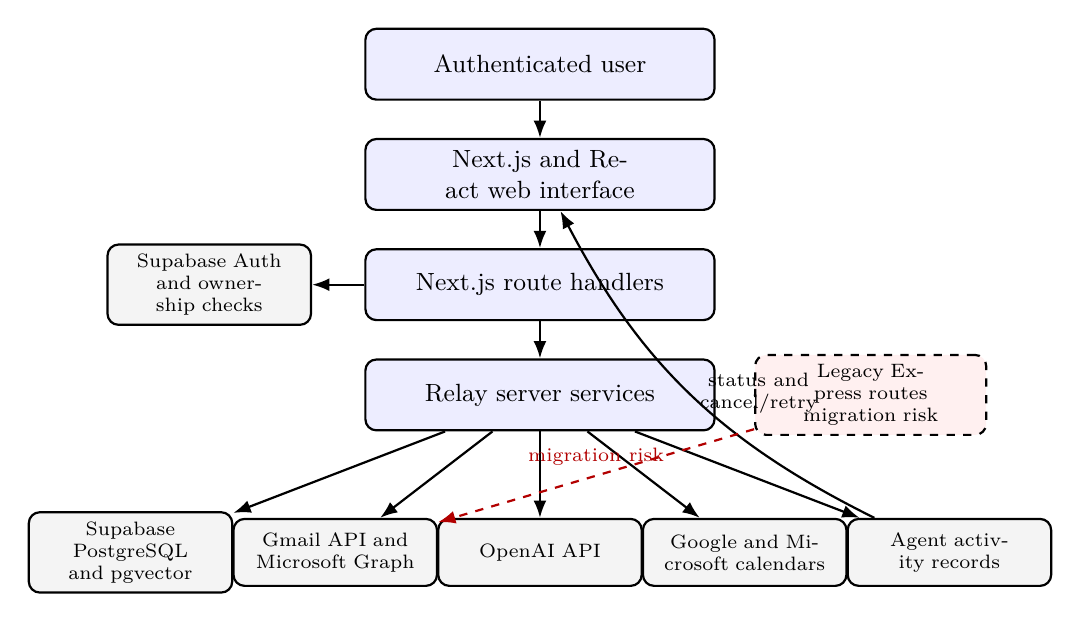
\begin{tikzpicture}[
  >={Latex[length=2.2mm]},
  relaybox/.style={draw, rounded corners, fill=blue!7, align=center,
    minimum height=0.9cm, text width=4.2cm, font=\small},
  service/.style={draw, rounded corners, fill=gray!9, align=center,
    minimum height=0.85cm, text width=2.35cm, font=\scriptsize},
  risk/.style={draw, dashed, rounded corners, fill=red!6, align=center,
    minimum height=0.85cm, text width=2.7cm, font=\scriptsize},
  every path/.style={draw, ->, thick}
]
  \node[relaybox] (user) at (0,4.2) {Authenticated user};
  \node[relaybox] (ui) at (0,2.8) {Next.js and React web interface};
  \node[relaybox] (api) at (0,1.4) {Next.js route handlers};
  \node[service] (auth) at (-4.2,1.4) {Supabase Auth and ownership checks};
  \node[relaybox] (core) at (0,0) {Relay server services};
  \node[service] (db) at (-5.2,-2.0) {Supabase PostgreSQL and pgvector};
  \node[service] (mail) at (-2.6,-2.0) {Gmail API and Microsoft Graph};
  \node[service] (openai) at (0,-2.0) {OpenAI API};
  \node[service] (calendar) at (2.6,-2.0) {Google and Microsoft calendars};
  \node[service] (activity) at (5.2,-2.0) {Agent activity records};
  \node[risk] (legacy) at (4.2,0) {Legacy Express routes\\migration risk};

  \path (user) -- (ui);
  \path (ui) -- (api);
  \path (api) -- (auth);
  \path (api) -- (core);
  \path (core) -- (db);
  \path (core) -- (mail);
  \path (core) -- (openai);
  \path (core) -- (calendar);
  \path (core) -- (activity);
  \path (activity) to[bend left=18] node[right, font=\scriptsize,
    align=center]{status and\\cancel/retry} (ui);
  \path[dashed, red!70!black] (legacy) -- node[above, font=\scriptsize]{migration risk} (mail);
\end{tikzpicture}
\caption{Relay high-level architecture and principal trust boundaries.}
\label{fig:relay-architecture}
\end{figure}

The browser is untrusted and receives only data intended for the
signed-in user. Next.js routes authenticate the session, validate
inputs, resolve account ownership, and call server-only services. Those
services interact with Supabase, providers, and OpenAI. Service-role
credentials, provider tokens, encryption keys, OAuth secrets, and the
OpenAI key remain server-side. The legacy Express layer is shown
separately because it is not the desired public trust boundary.

\section{3.3 Major Components}\label{33-major-components}

\begin{longtable}[]{@{}p{0.17\textwidth}p{0.27\textwidth}p{0.22\textwidth}p{0.26\textwidth}@{}}
\toprule\noalign{}
Component & Responsibility & Principal inputs & Principal outputs \\
\midrule\noalign{}
\endhead
\bottomrule\noalign{}
\endlastfoot
Application shell and mailbox UI & Navigation, account scope, mail
lists, reading, composing, responsive layout & Session, account
selection, API responses & User interactions and authenticated
requests \\
Authentication and account services & Validate Relay identity, OAuth
state, provider ownership, and token lifecycle & Bearer session, OAuth
callback, account ID & Authenticated user and usable provider client \\
Gmail and Outlook adapters & Normalize provider-specific fetch, sync,
thread, draft, send, and modification behavior & Account-scoped provider
IDs and operations & Normalized message data or provider result \\
AI routes and context assembly & Build prompts, select account/contact
context, validate structured results & User request, thread references,
settings, retrieved context & Summary, answer, draft, brief, or tool
proposal \\
Mailbox context & Combine selected thread, same-contact history,
accepted memory, and semantic chunks & User/account, selected message,
query, optional contact & Bounded context and source descriptors \\
Personalization and memory & Assemble preferences and learn reviewable
observations & Explicit settings, accepted memory, successful send
feedback & Bounded personalization context and memory items \\
Workflow activity & Record calendar, commitment, monitor, and brief work
& Authenticated workflow request and input & State, event history,
result, cancellation, or retry \\
Commitments and calendar & Track obligations, reminders, monitors,
events, and meeting briefs & User actions and selected email evidence &
User-owned commitments, events, and briefs \\
Target approval executor & Proposed extension binding reviewed payload
to later execution & Immutable proposal, expiry, user decision &
Approved execution, rejection, expiry, or failure record \\
\end{longtable}

\section{3.4 Data Design}\label{34-data-design}

The relational schema groups identity/preferences, provider mail,
AI/retrieval, memory, agent activity, commitments, and calendar data.
Provider identifiers remain beside normalized records so Relay can
return to source truth. User-owned rows carry \texttt{user\_id} or
derive ownership through a parent. Foreign keys and uniqueness
constraints reduce duplication, while RLS reinforces server
authorization. Because the service role can bypass RLS, routes must
still authenticate users and filter by ownership. Figure
\ref{fig:relay-er} shows the core logical relationships; Appendix C lists
additional supporting tables.

\begin{figure}[htbp]
\centering
\resizebox{\textwidth}{!}{%
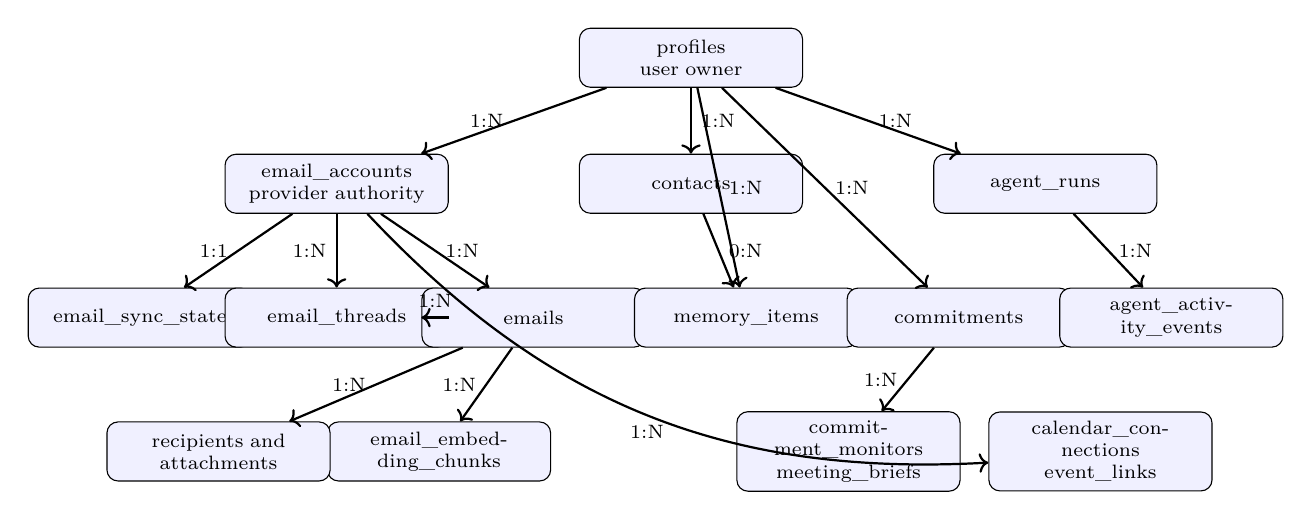
\begin{tikzpicture}[
  entity/.style={draw, rounded corners, fill=blue!6, align=center,
    minimum height=0.75cm, text width=2.6cm, font=\scriptsize},
  rel/.style={draw, ->, thick, font=\scriptsize}
]
  \node[entity] (profile) at (0,4.8) {profiles\\user owner};
  \node[entity] (account) at (-4.5,3.2) {email\_accounts\\provider authority};
  \node[entity] (contact) at (0,3.2) {contacts};
  \node[entity] (runs) at (4.5,3.2) {agent\_runs};
  \node[entity] (sync) at (-7.0,1.5) {email\_sync\_state};
  \node[entity] (threads) at (-4.5,1.5) {email\_threads};
  \node[entity] (emails) at (-2.0,1.5) {emails};
  \node[entity] (memory) at (0.7,1.5) {memory\_items};
  \node[entity] (commit) at (3.4,1.5) {commitments};
  \node[entity] (events) at (6.1,1.5) {agent\_activity\_events};
  \node[entity] (chunks) at (-3.2,-0.2) {email\_embedding\_chunks};
  \node[entity] (attach) at (-6.0,-0.2) {recipients and\\attachments};
  \node[entity] (monitor) at (2.0,-0.2) {commitment\_monitors\\meeting\_briefs};
  \node[entity] (cal) at (5.2,-0.2) {calendar\_connections\\event\_links};
  \draw[rel] (profile) -- node[left]{1:N} (account);
  \draw[rel] (profile) -- node[right]{1:N} (contact);
  \draw[rel] (profile) -- node[right]{1:N} (runs);
  \draw[rel] (account) -- node[left]{1:1} (sync);
  \draw[rel] (account) -- node[left]{1:N} (threads);
  \draw[rel] (account) -- node[right]{1:N} (emails);
  \draw[rel] (threads) -- node[above]{1:N} (emails);
  \draw[rel] (emails) -- node[left]{1:N} (chunks);
  \draw[rel] (emails) -- node[left]{1:N} (attach);
  \draw[rel] (profile) -- node[right]{1:N} (memory);
  \draw[rel] (contact) -- node[right]{0:N} (memory);
  \draw[rel] (profile) -- node[right]{1:N} (commit);
  \draw[rel] (commit) -- node[left]{1:N} (monitor);
  \draw[rel] (runs) -- node[right]{1:N} (events);
  \draw[rel] (account) to[bend right=25] node[below]{1:N} (cal);
\end{tikzpicture}}
\caption{Core logical entity-relationship diagram. Settings and auxiliary tables are omitted for readability.}
\label{fig:relay-er}
\end{figure}

\section{3.5 Retrieval and Context
Flow}\label{35-retrieval-and-context-flow}

\begin{figure}[htbp]
\centering
\begin{tikzpicture}[
  >={Latex[length=2.2mm]},
  step/.style={draw, rounded corners, fill=blue!6, align=left,
    minimum height=0.8cm, text width=11.8cm, font=\small},
  every path/.style={draw, ->, thick}
]
  \node[step] (s1) {\textbf{1. User request:} Open a thread or request AI help in an explicit account scope.};
  \node[step, below=0.45cm of s1] (s2) {\textbf{2. Authenticated route:} Validate the Relay user and resolve account ownership.};
  \node[step, below=0.45cm of s2] (s3) {\textbf{3. Selected evidence:} Fetch the exact provider thread when the request identifies a message.};
  \node[step, below=0.45cm of s3] (s4) {\textbf{4. Personalization:} Read accepted memory, same-contact sent mail, and scoped embedding matches.};
  \node[step, below=0.45cm of s4] (s5) {\textbf{5. Model context:} Separate trusted instructions from bounded, untrusted evidence.};
  \node[step, below=0.45cm of s5] (s6) {\textbf{6. User response:} Return a structured answer, summary, draft, brief, and source categories.};
  \path (s1) -- (s2);
  \path (s2) -- (s3);
  \path (s3) -- (s4);
  \path (s4) -- (s5);
  \path (s5) -- (s6);
\end{tikzpicture}
\caption{Implemented selected-thread and personalization context flow.}
\label{fig:retrieval-flow}
\end{figure}

This implemented flow limits context to an authenticated account and
keeps provider content as evidence rather than system instruction. Exact
selected threads and semantic context remain separate inputs; a future
general retrieval service should re-fetch semantic candidates before
treating them as current evidence.

\section{3.6 Workflow State and Target Approval
State}\label{36-workflow-state-and-target-approval-state}

\begin{figure}[htbp]
\centering
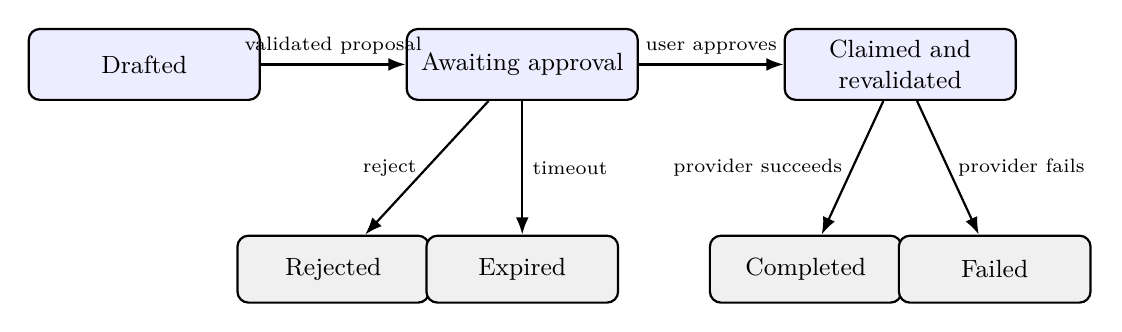
\begin{tikzpicture}[
  >={Latex[length=2.2mm]},
  state/.style={draw, rounded corners, fill=blue!7, align=center,
    minimum height=0.9cm, text width=2.7cm, font=\small},
  terminal/.style={draw, rounded corners, fill=gray!12, align=center,
    minimum height=0.85cm, text width=2.2cm, font=\small},
  every path/.style={draw, ->, thick}
]
  \node[state] (drafted) at (-4.8,1.6) {Drafted};
  \node[state] (awaiting) at (0,1.6) {Awaiting approval};
  \node[state] (claimed) at (4.8,1.6) {Claimed and revalidated};
  \node[terminal] (rejected) at (-2.4,-1.0) {Rejected};
  \node[terminal] (expired) at (0,-1.0) {Expired};
  \node[terminal] (completed) at (3.6,-1.0) {Completed};
  \node[terminal] (failed) at (6.0,-1.0) {Failed};

  \path (drafted) -- node[above, font=\scriptsize]{validated proposal} (awaiting);
  \path (awaiting) -- node[above, font=\scriptsize]{user approves} (claimed);
  \path (awaiting) -- node[left, font=\scriptsize]{reject} (rejected);
  \path (awaiting) -- node[right, font=\scriptsize]{timeout} (expired);
  \path (claimed) -- node[left, font=\scriptsize]{provider succeeds} (completed);
  \path (claimed) -- node[right, font=\scriptsize]{provider fails} (failed);
\end{tikzpicture}
\caption{Target approval state transitions for consequential model-proposed actions.}
\label{fig:approval-state}
\end{figure}

This is the target approval design. The baseline implements user-owned
\texttt{agent\_runs}, activity events, scheduling and terminal states,
idempotency fields, and authenticated cancel/retry. It does not implement
the complete approve, claim, immutable-payload revalidation, and execute
path. That path is required before consequential model-proposed actions
can be described as approval-gated.

\section{3.7 Deployment Design}\label{37-deployment-design}

The repository combines a Next.js application, a legacy Express process,
and a scheduled commitment job. Supabase, Gmail, Microsoft Graph,
OpenAI, and calendar systems are external services. Environment
variables keep service-role, provider, encryption, cron, and OpenAI
secrets server-side. CI targets Node.js 22 with quality, browser, and
security jobs. One primary web deployment owns session-aware routes and
services; scheduled work calls a secret-protected job endpoint. The
legacy Express process must be removed or private before release.

\section{3.8 Design Evolution}\label{38-design-evolution}

The architecture became more focused during implementation. Next.js
route handlers replaced the public SPA/Express boundary, Gmail history
and Outlook delta pulls replaced webhook dependencies, and OpenAI became
the implemented model provider. Provider search and scoped semantic
context replaced the originally unified FTS/RAG vision. Concrete
calendar, commitment, brief, and activity workflows were delivered
before the generic approval executor. The data model expanded, while the
privacy requirement was clarified to disclose minimized OpenAI
processing. The complete comparison table and rationale are maintained
in the public-ready System Design Document {[}21{]}.

\begin{center}\rule{0.5\linewidth}{0.5pt}\end{center}

\chapter{4. Alternative Designs}\label{4-alternative-designs}

\section{4.1 Separate SPA and Express API Versus Next.js
Backend-for-Frontend}\label{41-separate-spa-and-express-api-versus-nextjs-backend-for-frontend}

A conventional option was a React single-page application with an
independent Express REST API. This separation can support multiple
clients and independent scaling. It also creates two deployment units, a
broader CORS surface, duplicated routing conventions, and more
opportunities to pass tokens between browser and service.
Relay\textquotesingle s early backend work and remaining Express server
reflect this direction.

The selected direction places the user-facing API in authenticated
Next.js route handlers. UI and server boundaries remain distinct in
code, but share types, deployment, and session conventions. This is
simpler for a capstone team and fits the backend-for-frontend use case.
It is not a claim that monolithic deployment is universally superior. If
Relay later supports mobile or third-party clients, a separate versioned
service API may become appropriate. For the current web application, the
residual Express routes should be removed or network-isolated because
they complicate the trust model.

\section{4.2 Modular Monolith Versus
Microservices}\label{42-modular-monolith-versus-microservices}

Microservices could isolate synchronization, AI, calendar, and memory
workloads and scale them independently. They would also require service
authentication, distributed tracing, message delivery, deployment
automation, and operational maturity that exceed the
capstone\textquotesingle s demonstrated needs. Most user operations
share identity and account scope, making premature distribution a source
of risk.

Relay therefore uses a modular monolith: UI routes, API routes, and
server services are separate modules inside one primary application.
Background commitment processing is logically separate and
cron-authenticated. The design can later extract synchronization or
long-running AI work if measurements justify it. Extraction should
follow observed capacity or reliability limits, not fashion.

\section{4.3 Provider-Only Access Versus Local
Synchronization}\label{43-provider-only-access-versus-local-synchronization}

A provider-only design would fetch every view directly from Gmail or
Outlook. It minimizes local copies but increases latency, rate-limit
exposure, and provider-specific branching. A full mirror improves search
and offline analysis but expands retention, deletion, and consistency
obligations.

Relay chooses bounded synchronization plus provider grounding. Local
metadata, snapshots, and selected excerpts enable responsive listing and
retrieval. Exact provider content is fetched when a result must support
an answer or action. This hybrid approach accepts complexity in exchange
for speed and provenance. Retention and deletion still require
operational verification.

\section{4.4 Single-Shot AI Versus Retrieval and
Tools}\label{44-single-shot-ai-versus-retrieval-and-tools}

A single completion request containing the current thread is easy to
implement. It performs poorly when relevant context lies elsewhere and
cannot safely manipulate mailbox state. Sending a very large mailbox
context would increase cost and privacy exposure.

Relay selected task-specific structured outputs and bounded,
user-scoped context rather than sending a mailbox to one completion.
Implemented routes produce summaries, drafts, briefs, and
personalization results. A generalized multi-round tool runtime with
enforced read/write budgets was designed but is not in the baseline.

\section{4.5 Autonomous Writes Versus Approval-Gated
Actions}\label{45-autonomous-writes-versus-approval-gated-actions}

Direct autonomous writes would create a smoother interaction but an
unacceptable authorization model. Relay\textquotesingle s target design
separates preparation from execution: read-only assistance and drafts
can return immediately, while high-impact model proposals require
approval. The baseline has user-owned activity state, idempotency
metadata, concrete calendar/commitment workflows, and cancel/retry, but
the generic approval-and-execute path is incomplete.

\section{4.6 Knowledge Graph Versus Scoped Memory
Ledger}\label{46-knowledge-graph-versus-scoped-memory-ledger}

A broad knowledge graph could represent people, organizations, projects,
threads, and inferred relationships. It would support multi-hop
reasoning but would also make inference provenance, correction, and
sensitive-data control more difficult. The implemented choice is a
scoped memory ledger combined with contacts, snapshots, explicit
relational records, and retrieval. Memories have status, scope,
confidence, evidence, sensitivity, expiry, and contradiction
information. A lightweight graph remains future work for source-backed,
reviewable relationships only.

\begin{center}\rule{0.5\linewidth}{0.5pt}\end{center}

\chapter{5. Implementation}\label{5-implementation}

\section{5.1 Technology Stack and
Strategy}\label{51-technology-stack-and-strategy}

Relay is written primarily in TypeScript. The reviewed
\texttt{package.json} specifies Next.js 16.2.6, React 19.2.0, Supabase
JavaScript 2.107.0, Express 5.2.1, Zod 3.25.76, Tailwind CSS 4, Jest 29,
and Playwright 1.61.0. Development proceeded iteratively through feature
branches and pull requests. The stack supports shared types, component
testing, server-side provider clients, and schema-validated AI outputs.

The implementation strategy separates browser components from
server-only modules. The \texttt{app} directory contains pages and route
handlers. Reusable UI resides in \texttt{components}. Provider,
authentication, AI, personalization, memory, commitment, calendar,
encryption, and activity logic resides under \texttt{lib/server}.
Supabase SQL defines the target schema and incremental migrations. Tests
are grouped by contract, unit, integration, performance, and end-to-end
scope. Low-level responsibilities and interfaces are recorded in the
System Design Document {[}21{]}.

\section{5.2 Frontend Implementation}\label{52-frontend-implementation}

The interface uses desktop and mobile navigation, with account selection
establishing mailbox and AI scope. Shared modules support inbox, sent,
drafts, archives, trash, thread, search, and compose views. Assistants
expose summaries, questions, tasks, briefs, and drafts beside relevant
messages. Other pages cover chat history, activity, calendar,
commitments, meeting briefs, and settings. Chat can stream answers,
sources, tool status, clarification, drafts, and approval cards, making
workflow state visible.

Responsive components and mobile navigation support smaller screens.
DOMPurify is available for sanitizing rendered HTML. However, the
existence of responsive code and sanitization libraries is not
equivalent to a completed accessibility or cross-browser audit. Those
claims require manual evidence.

\section{5.3 Authentication and Provider
Accounts}\label{53-authentication-and-provider-accounts}

Relay users authenticate through Supabase. Server routes validate the
bearer session and derive the trusted user identifier rather than
accepting ownership from the model or request body. Gmail and Outlook
OAuth callbacks associate encrypted provider credentials with an
\texttt{email\_accounts} row. The provider account includes its type,
provider identity, token expiry, and sync state.

Gmail services parse metadata and MIME content, handle attachments,
create drafts, send mail, and apply mailbox changes. Outlook services
use Microsoft Graph for equivalent supported operations and normalize
their results. A provider-neutral email API lets components request
messages without implementing two complete clients. Provider-specific
constraints remain visible; for example, Gmail categories are not
applied to Outlook-only inboxes.

Token encryption uses AES-256-GCM with a fresh initialization vector and
authentication tag. OAuth state is encrypted and carries issuance
information so expired state can be rejected. A compatibility path can
read legacy plaintext tokens, which is useful for migration but should
be eliminated after all stored credentials are re-encrypted.

\section{5.4 Mail Synchronization, Search, and
Attachments}\label{54-mail-synchronization-search-and-attachments}

Synchronization stores account-scoped message/thread metadata and
provider cursors, with constraints against duplicate messages and
drafts. Recipients, attachments, and labels are normalized. Cursor
pagination avoids loading a mailbox at once. HTML, plain text, and
attachments remain untrusted. Performance tests guard parsing and
encoding regressions but are not capacity benchmarks; live sync at
meaningful mailbox sizes remains planned.

\section{5.5 Contextual AI}\label{55-contextual-ai}

Server-side OpenAI integration supports structured thread summaries,
tasks, draft replies, inbox briefs, and meeting support. Chat-session
tables and routes persist conversation metadata, but the baseline does
not expose the generalized mailbox-chat agent route from the broader
vision. Zod schemas constrain requests and model responses. Settings and
per-account preferences remain server-controlled.

Context assembly combines account preferences, explicit profile
information, accepted memories, recent context, contact information,
sent messages to the same contact, relevant mailbox evidence, and active
commitments. Each source is bounded. Responses include context-source
metadata where supported, allowing the interface to show what kinds of
information influenced an answer. Raw unrelated email is not displayed
merely because it was considered during retrieval.

\section{5.6 Hybrid Mailbox
Retrieval}\label{56-hybrid-mailbox-retrieval}

The personalization service builds user- and account-scoped context.
Optional embeddings use \texttt{match\_email\_embedding\_chunks};
same-contact sent mail and accepted memory remain available when
embeddings fail. Exact provider content is loaded for a thread the user
selected. Separately, email search queries Gmail or Outlook and caches
normalized metadata where appropriate. These paths do not yet form the
complete generalized hybrid service: automatic re-fetch of semantic
candidates, unified database FTS/vector results, and automatic provider
fallback remain incomplete.

\section{5.7 Memory and
Personalization}\label{57-memory-and-personalization}

\texttt{memory\_items} stores reviewable observations with category,
scope, activation state, sensitivity, confidence, evidence count,
timestamps, expiry, and contradiction metadata. Quality functions
canonicalize text, generate fingerprints for deduplication, detect
secret-like or sensitive patterns, and enforce activation thresholds.
Explicit low-risk observations require confidence of at least 0.85 for
automatic activation. Inferred workflow or style observations require
confidence of at least 0.80 and two pieces of evidence. Sensitive
observations remain quarantined for review.

\texttt{draft\_feedback} compares generated and final sent text after a
successful provider send. Repeated edits may suggest a preference such
as greeting, tone, or signoff. The memory UI lets users correct or
remove what Relay learned. Maintenance compacts active style preferences
and ignores inactive, expired, archived, rejected, or contradicted
memories. Embedding or learning failure must not block ordinary sending.

\section{5.8 Commitments, Calendar, and
Briefs}\label{58-commitments-calendar-and-briefs}

Users can create, complete, reopen, dismiss, snooze, and monitor
commitments. A cron-authenticated route processes background jobs.
Google and Microsoft calendar connections link workflow state to
provider events, while meeting briefs collect preparation context. These
features turn email into tracked action and make ownership, idempotency,
expiry, audit, and approval essential.

\section{5.9 Workflow Activity and Approval
Foundation}\label{59-workflow-activity-and-approval-foundation}

Relay implements durable \texttt{agent\_runs} and
\texttt{agent\_activity\_events} for commitment monitors, calendar work,
and meeting briefs. Runs carry ownership, state, scheduling, input and
output manifests, attempt count, and optional idempotency key. Users can
inspect events, cancel eligible work, or retry failed, partial, or
cancelled work. The baseline lacks a general immutable proposal,
explicit approval, atomic claim, revalidation, and execution route;
email writes remain authenticated user-directed operations.

\section{5.10 Low-Level Implementation
Flows}\label{510-low-level-implementation-flows}

Low-level implementation follows a server-owned pattern: authenticate,
resolve an owned account, validate bounded input, call the provider or
domain service, persist user-scoped results, and return a controlled
response. OAuth adds encrypted expiring state and tokens; Gmail uses
history cursors; Outlook uses delta links; AI routes add bounded
personalization and schema validation; successful sends can add filtered
draft feedback; workflow routes add activity events and state checks.
Appendix B and {[}21{]} provide the detailed flow table.

\section{5.11 Implementation Evolution and
Challenges}\label{511-implementation-evolution-and-challenges}

Challenges included preserving provider differences, explicit account
scope, useful context under partial sync, safe memory, and evolving a
broad agent vision into testable workflows. The team replaced the
SPA/Express boundary with Next.js routes, webhook-dependent sync with
history/delta polling, narrowed AI support to OpenAI, and implemented
activity history before the full approval executor. These are recorded
scope and risk decisions rather than hidden omissions.

\begin{center}\rule{0.5\linewidth}{0.5pt}\end{center}

\chapter{6. Testing and Evaluation}\label{6-testing-and-evaluation}

\section{6.1 Testing Objectives}\label{61-testing-objectives}

Testing targets correctness, user/account isolation, provider
normalization, safe AI orchestration, schema constraints, and
regressions. Critical failures include unauthorized access, token
exposure, incorrect modification, synchronization errors, context
leakage, unsafe actions, and corrupted memory. The Relay QA strategy
{[}3{]} uses Jest {[}18{]}, React Testing Library, Playwright {[}19{]},
TypeScript, ESLint, GitHub Actions {[}20{]}, CodeQL, and dependency
audit. Evidence is stronger for automated logic than for production,
usability, or load behavior.

\section{6.2 Automated Test Layers}\label{62-automated-test-layers}

\begin{itemize}
\tightlist
\item
  \textbf{Unit tests} cover email parsing and formatting, Gmail and
  Outlook adapters, encryption, authentication helpers, AI rate limits,
  memory quality, personalization, pagination, provider accounts, and
  computer-use URL restrictions.
\item
  \textbf{Component tests} cover authentication state, account
  selection, navigation, search, inbox and thread interactions, compose
  behavior, AI markdown, assistant interfaces, and responsive shell
  elements.
\item
  \textbf{Integration tests} invoke API route logic with Gmail, Outlook,
  Supabase, and OpenAI dependencies mocked. They test authentication,
  ownership, request validation, response shaping, and agent activity.
\item
  \textbf{Schema-contract tests} statically inspect SQL for RLS,
  ownership policies, provider checks, and uniqueness constraints. They
  do not start PostgreSQL or prove the migrations in a live Supabase
  project.
\item
  \textbf{Performance-regression tests} use generous time budgets for
  selected parsing and encoding operations. They identify major
  regressions but do not measure capacity or end-user latency.
\item
  \textbf{End-to-end tests} define Playwright authentication smoke flows
  against a production build. Authenticated provider workflows require
  controlled test accounts and secrets and are intentionally separated
  from untrusted pull-request jobs.
\end{itemize}

\section{6.3 Verified Results}\label{63-verified-results}

On August 11, 2026, the Jest command completed with \textbf{36 passing
test suites and 206 passing tests}. No Jest snapshot tests were present.
Coverage generated by the configured scope was:

\begin{longtable}[]{@{}p{0.28\textwidth}p{0.12\textwidth}p{0.12\textwidth}p{0.22\textwidth}@{}}
\toprule\noalign{}
Metric & Covered & CI threshold & Result \\
\midrule\noalign{}
\endhead
\bottomrule\noalign{}
\endlastfoot
Statements & 100\% & 100\% & Passed \\
Branches & 100\% & 100\% & Passed \\
Functions & 100\% & 100\% & Passed \\
Lines & 100\% & 100\% & Passed \\
\end{longtable}

Coverage is intentionally collected from a defined set of core UI and
server modules, not every repository file. The 100\% result covers every
instrumented statement, branch, function, and line in that configured
scope, including the shared email API, encryption, Gmail parsing,
authentication helpers, and selected components. It does not claim
100\% coverage across all production files, live provider behavior, or
deployed infrastructure.

\section{6.4 Representative Test
Cases}\label{64-representative-test-cases}

\begin{longtable}[]{@{}p{0.28\textwidth}p{0.35\textwidth}p{0.29\textwidth}@{}}
\toprule\noalign{}
Test scenario & Expected result & Evidence status \\
\midrule\noalign{}
\endhead
\bottomrule\noalign{}
\endlastfoot
Decrypt a token after AES-GCM encryption & Original plaintext is
restored & Automated Jest pass \\
Modify an encrypted payload & Authentication fails and tampering is
rejected & Automated Jest pass \\
Call account API without valid user & Request is rejected & Automated
integration pass \\
Return connected accounts & Provider tokens are excluded from the API
response & Automated integration pass \\
Inspect user-owned SQL tables & RLS and ownership policies are present &
Static contract pass \\
Exceed AI request allowance & Controlled rate-limit response is returned
& Automated Jest pass \\
Cancel another user\textquotesingle s activity or retry an ineligible
run & Ownership or state validation rejects the operation & Automated
agent-activity integration pass \\
Supply an unsafe computer-use start URL & Destination validation rejects
it & Automated Jest pass \\
Load login page and validate credentials in browser & Expected UI and
validation behavior & Automated Playwright pass (3 smoke tests) \\
Synchronize two real users across Gmail and Outlook & No account or
provider leakage & Manual staging evidence required \\
\end{longtable}

\section{6.5 Continuous Integration}\label{65-continuous-integration}

The GitHub Actions workflow defines three jobs. The quality job installs
dependencies, runs ESLint, TypeScript, Jest with coverage, and a
production build. The browser job installs Chromium, builds, and runs
Playwright. The security job performs a high-severity dependency audit
and CodeQL JavaScript/TypeScript analysis; CodeQL analysis is currently
non-blocking until code scanning is enabled. Coverage is uploaded as a
workflow artifact.

\section{6.6 Evaluation Limitations}\label{66-evaluation-limitations}

The repository does not establish a completed user study, production
telemetry, accessibility audit, provider-scale load test, or external
penetration test. Mocked integration tests intentionally avoid live user
data and secrets. Static SQL contracts do not prove deployed RLS.
Playwright coverage focuses on unauthenticated smoke behavior unless
controlled accounts are configured. AI quality tests validate
orchestration more readily than semantic correctness, hallucination
rate, or user trust.

\begin{center}\rule{0.5\linewidth}{0.5pt}\end{center}

\chapter{7. Security}\label{7-security}

\section{7.1 Security Objectives and
Assets}\label{71-security-objectives-and-assets}

Relay\textquotesingle s security objectives are confidentiality of
private email and tokens, integrity of user-approved actions and stored
context, availability of core workflows, and strict separation between
users and connected accounts. Sensitive assets include Supabase
sessions, OAuth access and refresh tokens, encryption and service-role
keys, message and attachment content, contacts, calendar data, AI
prompts and outputs, memory records, approvals, logs, backups, and
deployment configuration.

The Relay Security Plan {[}5{]} is a risk-based plan and repository
review, not a completed penetration-test report. It identifies current
controls, open gaps, staging rules, evidence requirements, severity,
ownership, re-test, and release criteria. This thesis preserves that
distinction.

\section{7.2 Trust Boundaries and
Threats}\label{72-trust-boundaries-and-threats}

The browser, user-entered text, emails, attachments, calendar
descriptions, contact names, retrieved memory, provider results,
webpages, and model outputs are untrusted. External providers are
trusted to perform their documented service but are outside the
team\textquotesingle s infrastructure. The server is responsible for
converting an authenticated request into a narrowly scoped provider
action.

Principal threats include:

\begin{itemize}
\tightlist
\item
  stolen or exposed OAuth tokens;
\item
  broken user or account authorization;
\item
  SQL/filter, MIME-header, HTML, URL, or log injection;
\item
  unsafe file types and attachment processing;
\item
  direct or indirect prompt injection in email content;
\item
  cross-user retrieval or memory contamination;
\item
  model-generated tool arguments that exceed user intent;
\item
  approval replay, duplicate execution, or payload substitution;
\item
  server-side request forgery through browser/computer-use destinations;
\item
  denial of wallet through unbounded model or tool loops;
\item
  secrets or private bodies in logs, URLs, analytics, or error
  responses; and
\item
  missing transport, browser-header, retention, backup, and
  incident-response controls.
\end{itemize}

\section{7.3 Implemented Controls}\label{73-implemented-controls}

Authentication helpers validate the Supabase user at protected routes.
Server code supplies trusted user and account scope. Database RLS and
policy contracts provide defense in depth. Provider tokens are encrypted
with AES-256-GCM, and token values are excluded from account responses.
OAuth state includes integrity protection and age validation. Zod
schemas bound many request and structured output fields. Email HTML
display uses sanitization, and Gmail MIME generation has tests for
header-injection prevention.

Implemented AI controls include server-owned prompts, structured
response schemas, authenticated account resolution, bounded context,
rate limiting, and user-scoped memory with confidence, sensitivity,
evidence, activation, expiry, contradiction, and deletion controls.
Activity routes enforce ownership and state rules for cancellation and
retry. Model tool budgets, immutable approval payloads, expiry, atomic
claiming, and approval-time revalidation remain target controls.

These controls reduce risk but do not prove absence of vulnerabilities.
RLS must be tested against a deployed database, sanitization must be
evaluated in every output context, and prompts alone cannot prevent all
prompt injection.

\section{7.4 Open Risks and Required
Hardening}\label{74-open-risks-and-required-hardening}

The security review assigns the highest immediate concern to the legacy
Express OAuth and email routes. They require removal or network
isolation because they do not consistently share the authenticated
Next.js trust boundary and may pass provider tokens through
browser-visible channels. Computer-use destinations require scheme,
host, redirect, DNS, private-address, localhost, and metadata-endpoint
protection. Some routes require consistent Zod schemas, bounded
collections, MIME/magic checks, rate limits, and generic errors.

Authentication hardening remains incomplete in repository evidence.
Password reset, breached-password screening, MFA, enumeration
resistance, session policy, and rate-limit behavior must be verified
through the identity provider and deployed application. Browser security
headers such as a restrictive Content Security Policy, HSTS,
\texttt{nosniff}, referrer policy, permissions policy, framing
restrictions, and safe cache controls require deployment evidence.
Attachment quarantine or malware scanning is not demonstrated.

Operational gaps include a verified retention and deletion job, backup
restore test, logging review, incident response, key rotation, secret
scanning, deployment inventory, and production monitoring. These gaps
are reasons to avoid an external-release claim.

\section{7.5 Security Testing Plan}\label{75-security-testing-plan}

Security testing should use an isolated staging deployment, separate
Supabase project, at least two Relay users, multiple provider test
accounts, synthetic messages, and non-production keys. Tests should
cover unauthenticated, malformed, expired, revoked, and cross-user
tokens; two-user and two-account isolation; OAuth state replay; token
leakage; RLS for every operation; HTML and MIME injection; malicious
URLs; unsupported attachments; rate and size limits; prompt injection;
memory poisoning; tool escalation; approval replay; and delete/retention
verification.

CodeQL, dependency audit, unit tests, and schema contracts should run in
CI. Manual proxy testing and browser inspection should verify headers,
redirects, referrers, storage, and error bodies. AI red-team cases
should place hostile instructions in subjects, bodies, attachments,
calendars, contacts, memory candidates, and provider search results. A
pass requires that untrusted text cannot change account scope, authorize
a tool, or bypass approval.

\section{7.6 Release Criteria}\label{76-release-criteria}

Relay should not be externally deployed while a critical finding remains
open. Before release, every public route must have a documented
authentication and authorization rule; two-user isolation must pass;
current provider tokens and secrets must be absent from client
responses, URLs, and logs; destructive or external writes must require
revalidated approval; high-severity dependencies must be addressed or
formally accepted; and the final report must record scope, tools,
findings, fixes, re-tests, limitations, and a release decision.

\begin{center}\rule{0.5\linewidth}{0.5pt}\end{center}

\chapter{8. Results and Discussion}\label{8-results-and-discussion}

\section{8.1 Functional Outcomes}\label{81-functional-outcomes}

The repository implements Gmail and Outlook, normalized mail views and
actions, contextual thread/compose/brief assistance, multi-account
scope, calendar, commitments, meeting briefs, model settings,
chat-session persistence, memory review, semantic context, and activity
history. Generalized mailbox chat, automatic hybrid grounding, and
complete approval-gated model actions remain partial requirements.

\section{8.2 Quality Outcomes}\label{82-quality-outcomes}

The verified Jest result demonstrates breadth across server logic,
components, integrations, database contracts, and regression tests.
Coverage exceeded every configured threshold. Security-relevant paths
such as token encryption, tamper rejection, authentication helpers, RLS
contracts, MIME handling, rate limits, account ownership, and
agent-activity state behavior have automated coverage.

This evidence supports the conclusion that Relay is a substantial,
testable software system. It does not support a conclusion that every
integrated service works under production conditions. The test design
deliberately mocks live Gmail, Outlook, Supabase, and OpenAI calls in
normal pull-request execution to protect credentials and avoid modifying
real mailboxes. That trade-off is appropriate for CI but makes
controlled staging tests necessary.

\section{8.3 Design Trade-Offs}\label{83-design-trade-offs}

The modular monolith reduced operational overhead but concentrates
responsibility. Hybrid sync improves responsiveness while adding
retention work; grounding adds latency; reviewable memory learns more
slowly; and approval adds interaction. Technical debt includes legacy
Express routes, an unverified live migration sequence, limited semantic
AI evaluation, and planned memory capabilities that are not yet
implemented.

\section{8.4 Evaluation Against
Objectives}\label{84-evaluation-against-objectives}

\begin{longtable}[]{@{}p{0.20\textwidth}p{0.32\textwidth}p{0.40\textwidth}@{}}
\toprule\noalign{}
Objective & Baseline result & Interpretation \\
\midrule\noalign{}
\endhead
\bottomrule\noalign{}
\endlastfoot
Unified Gmail and Outlook workspace & Implemented in provider and UI
modules & Functional evidence exists; live final demo still required \\
Contextual AI assistance & Implemented across compose, thread, inbox,
meeting, and chat routes & Structured and source-aware; semantic
accuracy not formally measured \\
Retrieval-augmented context & Selected threads, same-contact history,
memory, and semantic chunks implemented & Generalized grounding/fallback
and recall benchmarks remain incomplete \\
Personalization memory & Reviewable memory quality and maintenance paths
implemented & Privacy-oriented; long-term user value not studied \\
Commitment and calendar workflow & Routes, services, schema, pages, and
cron design implemented & External provider and scheduled-operation
evidence required \\
User and account isolation & Authentication helpers, ownership filters,
RLS schema, and contracts implemented & Deployed two-user test remains
mandatory \\
Safe agent actions & User-owned activity and concrete calendar/commitment
workflows implemented & Generic approval/revalidation and adversarial
testing remain incomplete \\
Automated quality & 36 suites and 206 tests passed; 100\% coverage gates
met & Strong repository evidence within configured scope \\
Production readiness & Not established & Security, load, accessibility,
operations, and user evidence incomplete \\
\end{longtable}

\section{8.5 Overall Discussion}\label{85-overall-discussion}

Relay applies frontend design, provider APIs, authentication, relational
data, AI orchestration, retrieval, security, automation, and CI to a
complex integration problem. Its strongest contribution is treating
email as evidence rather than authority. Code and tests show implemented
behavior, but production readiness depends on live configuration and
controlled validation. Relay is therefore a substantial security-aware
capstone prototype, not a certified production email service.

\begin{center}\rule{0.5\linewidth}{0.5pt}\end{center}

\chapter{9. Conclusion and Future
Work}\label{9-conclusion-and-future-work}

\section{9.1 Conclusion}\label{91-conclusion}

This project designed and implemented Relay, a unified communication
workspace for Gmail and Outlook with AI assistance, calendar and
commitment workflows, personalization memory, semantic retrieval, and
activity-tracked work. The system evolved from a communication backend
into an account-scoped assistant platform. Its modular services,
relational ownership, selected-thread context, and correctable memory
address important risks. The generalized approval-gated executor remains
a documented next step rather than a completed result.

Automated evidence is meaningful: 206 Jest tests across 36 suites
passed, and the configured core-module scope reached the enforced 100\%
thresholds for statements, branches, functions, and lines. The project
also maintains QA, memory-architecture, changelog, and security-plan
documentation. At the same time, the team has not used those artifacts
to hide limitations. Live multi-provider behavior, deployed RLS,
accessibility, user outcomes, scale, and security closure require
additional evidence.

The engineering lesson is that useful agent behavior depends as much on
boundaries as capability. Retrieval needs provenance. Personalization
needs correction and expiry. A model needs strict tools and limits.
Approval needs an immutable payload and ownership revalidation. These
principles make Relay a stronger foundation for continued development.

\section{9.2 Team Retrospective and Professional
Growth}\label{92-team-retrospective-and-professional-growth}

From the team\textquotesingle s perspective, Relay required us to work
through an evolving scope while keeping the project understandable to
people responsible for different areas. We divided ownership according
to each member\textquotesingle s strengths, used shared documentation
and version control to coordinate changes, and reviewed progress at
regular checkpoints. As integrations and quality requirements expanded,
some tasks took longer than first estimated and occasionally required
redistribution. This highlighted the value of smaller deliverables,
clearer acceptance criteria, and earlier communication when one area
depended on another. The team became more consistent at recording
decisions and identifying what was completed, partial, or dependent on
external evidence.

The project also supported professional growth beyond individual
implementation tasks. We improved at explaining design decisions,
reviewing one another\textquotesingle s work, responding constructively
to feedback, and balancing desired features against time, security, and
testing constraints. Working across interface, data, integration, AI,
testing, and documentation concerns reinforced that software engineering
is collaborative rather than a collection of isolated contributions. A
major lesson was that a credible result depends on clear boundaries and
honest evidence as much as visible functionality. If the project
continued, we would establish measurable completion criteria earlier,
schedule integration checks sooner, and preserve more time for user
evaluation and final operational validation.

\section{9.3 Prioritized Future Work}\label{93-prioritized-future-work}

\begin{enumerate}
\def\labelenumi{\arabic{enumi}.}
\tightlist
\item
  \textbf{Close release-blocking security risks:} remove or isolate
  legacy Express routes, complete destination controls, normalize
  validation and rate limits, configure security headers, and execute
  the security test plan.
\item
  \textbf{Validate the real environment:} apply every migration to a
  staging Supabase project and run two-user, two-account Gmail and
  Outlook scenarios with synthetic data.
\item
  \textbf{Complete quality evidence:} run final Playwright, build,
  audit, CodeQL, accessibility, and browser checks and publish stable CI
  links.
\item
  \textbf{Benchmark performance and reliability:} measure mailbox sync
  sizes, inbox render time, retrieval latency, provider fallback, AI
  response time, error recovery, and concurrent use.
\item
  \textbf{Evaluate users responsibly:} conduct task-based usability
  sessions with documented consent, participant characteristics, success
  measures, and limitations.
\item
  \textbf{Improve deep personalization:} add source-backed personal
  records for bills, receipts, subscriptions, travel, appointments,
  deliveries, and warranties with confirmation for sensitive facts.
\item
  \textbf{Add inspectable relationships:} introduce lightweight entity
  and relationship records only where every edge has source, confidence,
  scope, review state, and deletion controls.
\item
  \textbf{Strengthen operations:} define monitoring, backup restore,
  retention, deletion, incident response, key rotation, and
  disaster-recovery procedures.
\end{enumerate}

\section{9.4 Closing Statement}\label{94-closing-statement}

Relay demonstrates that an AI email agent can be more than a text
generator. By unifying providers, grounding context, tracking
commitments, learning cautiously, and asking before it acts, the project
offers a practical model for personal communication software that
remains accountable to its user.

\begin{center}\rule{0.5\linewidth}{0.5pt}\end{center}

\chapter{References}\label{references}

{[}1{]} Relay Capstone Team, "Relay Agent Back repository," GitHub.
{[}Online{]}. Available:
\url{https://github.com/dmann001/Relay-agent-back}. Accessed: Aug. 5,
2026.

{[}2{]} Relay Capstone Team, "Relay changelog," GitHub. {[}Online{]}.
Available:
\url{https://github.com/dmann001/Relay-agent-back/blob/main/docs/CHANGELOG.md}.
Accessed: Aug. 5, 2026.

{[}3{]} Relay Capstone Team, "Relay testing strategy, quality assurance,
and CI/CD planning," GitHub. {[}Online{]}. Available:
\url{https://github.com/dmann001/Relay-agent-back/blob/main/docs/QA.md}.
Accessed: Aug. 5, 2026.

{[}4{]} Relay Capstone Team, "Relay personalization memory
architecture," GitHub. {[}Online{]}. Available:
\url{https://github.com/dmann001/Relay-agent-back/blob/main/docs/MEMORY_ARCHITECTURE.md}.
Accessed: Aug. 5, 2026.

{[}5{]} Relay Capstone Team, "Relay security plan," ver. 1.0, Jul. 24,
2026. {[}Online{]}. Available:
\url{https://github.com/dmann001/Relay-agent-back/blob/main/docs/Relay_Security_Plan.pdf}.
Accessed: Aug. 5, 2026.

{[}6{]} Meta Platforms, Inc., "React," React Documentation.
{[}Online{]}. Available: \url{https://react.dev/}. Accessed: Aug. 5,
2026.

{[}7{]} Vercel, Inc., "Next.js App Router and route handlers," Next.js
Documentation. {[}Online{]}. Available:
\url{https://nextjs.org/docs/app} and
\url{https://nextjs.org/docs/app/getting-started/route-handlers}.
Accessed: Aug. 5, 2026.

{[}8{]} Supabase, Inc., "Row Level Security," Supabase Documentation.
{[}Online{]}. Available:
\url{https://supabase.com/docs/guides/database/postgres/row-level-security}.
Accessed: Aug. 5, 2026.

{[}9{]} Google, "Gmail API overview," Google for Developers.
{[}Online{]}. Available:
\url{https://developers.google.com/workspace/gmail/api/guides}.
Accessed: Aug. 5, 2026.

{[}10{]} Google, "Implement server-side authorization," Google for
Developers. {[}Online{]}. Available:
\url{https://developers.google.com/workspace/gmail/api/auth/web-server}.
Accessed: Aug. 5, 2026.

{[}11{]} Microsoft, "Use the Outlook mail REST API," Microsoft Learn.
{[}Online{]}. Available:
\url{https://learn.microsoft.com/en-us/graph/api/resources/mail-api-overview?view=graph-rest-1.0}.
Accessed: Aug. 5, 2026.

{[}12{]} D. Hardt, "The OAuth 2.0 Authorization Framework," RFC 6749,
Internet Engineering Task Force, Oct. 2012. {[}Online{]}. Available:
\url{https://www.rfc-editor.org/rfc/rfc6749}. Accessed: Aug. 5, 2026.

{[}13{]} OpenAI, "Developer quickstart: Responses API and tools," OpenAI
API Documentation. {[}Online{]}. Available:
\url{https://platform.openai.com/docs/quickstart}. Accessed: Aug. 5,
2026.

{[}14{]} P. Lewis \emph{et al.}, "Retrieval-Augmented Generation for
Knowledge-Intensive NLP Tasks," in \emph{Advances in Neural Information
Processing Systems 33}, 2020. {[}Online{]}. Available:
\url{https://papers.neurips.cc/paper/2020/hash/6b493230205f780e1bc26945df7481e5-Abstract.html}.
Accessed: Aug. 5, 2026.

{[}15{]} E. Tabassi, "Artificial Intelligence Risk Management Framework
(AI RMF 1.0)," NIST AI 100-1, National Institute of Standards and
Technology, Jan. 2023. {[}Online{]}. Available:
\url{https://doi.org/10.6028/NIST.AI.100-1}. Accessed: Aug. 5, 2026.

{[}16{]} OWASP Foundation, "LLM Prompt Injection Prevention Cheat
Sheet," OWASP Cheat Sheet Series. {[}Online{]}. Available:
\url{https://cheatsheetseries.owasp.org/cheatsheets/LLM_Prompt_Injection_Prevention_Cheat_Sheet.html}.
Accessed: Aug. 5, 2026.

{[}17{]} OWASP Foundation, "AI Agent Security Cheat Sheet," OWASP Cheat
Sheet Series. {[}Online{]}. Available:
\url{https://cheatsheetseries.owasp.org/cheatsheets/AI_Agent_Security_Cheat_Sheet.html}.
Accessed: Aug. 5, 2026.

{[}18{]} Jest, "Getting started," Jest Documentation. {[}Online{]}.
Available: \url{https://jestjs.io/docs/getting-started}. Accessed: Aug.
5, 2026.

{[}19{]} Microsoft, "Installation," Playwright Documentation.
{[}Online{]}. Available: \url{https://playwright.dev/docs/intro}.
Accessed: Aug. 5, 2026.

{[}20{]} GitHub, Inc., "GitHub Actions documentation." {[}Online{]}.
Available: \url{https://docs.github.com/en/actions}. Accessed: Aug. 5,
2026.

{[}21{]} Relay Capstone Team, "Relay System Design Document," GitHub.
{[}Online{]}. Available:
\url{https://github.com/dmann001/Relay-agent-back/blob/main/docs/Relay_System_Design_Document.tex}.
Accessed: Aug. 11, 2026.

\begin{center}\rule{0.5\linewidth}{0.5pt}\end{center}

\chapter{Appendices}\label{appendices}

\section{Appendix A - Requirements
Traceability}\label{appendix-a---requirements-traceability}

\subsection{Original Functional Requirements Versus End Product}

\begin{longtable}[]{@{}p{0.06\textwidth}p{0.25\textwidth}p{0.36\textwidth}p{0.23\textwidth}@{}}
\toprule\noalign{}
ID & Original requirement & End-product implementation & Status/evolution \\
\midrule\noalign{}
\endhead
\bottomrule\noalign{}
\endlastfoot
FR-01 & Gmail/Outlook OAuth & Supabase user auth plus provider callbacks and encrypted tokens & Implemented; two trust steps \\
FR-02 & Multiple accounts & Account records, selector, scoped APIs, disconnect & Implemented \\
FR-03 & Synchronize connected accounts & Gmail history and Outlook delta pulls & Implemented; pulls replaced webhook dependencies \\
FR-04 & Unified inbox & Shared routes and provider-neutral records & Implemented \\
FR-05 & Complete threads & Provider-aware message/thread routes & Implemented \\
FR-06 & AI summaries & Thread assistant and brief routes & Implemented; quality study required \\
FR-07 & Context-aware drafts & Preferences, contact context, memory, selected mail & Implemented \\
FR-08 & FTS and vector search & Provider search plus semantic personalization chunks & Partial; unified FTS/vector endpoint absent \\
FR-09 & RAG and citations & Same-contact history, memory, chunks, selected threads & Partial; generalized grounding/citations incomplete \\
FR-10 & Agent proposals & Calendar, commitments, monitors, briefs, activity & Partial; generic proposal/label tool absent \\
FR-11 & Explicit confirmation & Activity states plus owned cancel/retry & Partial; approve-and-execute route required \\
FR-12 & Embedding storage & pgvector chunks, match function, hashes, indexes & Implemented; production recall/scale unverified \\
FR-13 & RLS isolation & Ownership columns, RLS SQL, constraints, contracts & Partial until deployed two-user test \\
\end{longtable}

\subsection{Original Non-Functional Requirements Versus End Product}

\begin{longtable}[]{@{}p{0.07\textwidth}p{0.24\textwidth}p{0.37\textwidth}p{0.22\textwidth}@{}}
\toprule\noalign{}
ID & Original group & End-product implementation & Status/evolution \\
\midrule\noalign{}
\endhead
\bottomrule\noalign{}
\endlastfoot
NFR-01 & Security & Encryption, OAuth, ownership checks, RLS SQL, validation & Partial; deployed headers/RLS and pen test needed \\
NFR-02 & Reliability & Token refresh, cursor recovery, soft AI failure, activity events & Partial; monitoring/backup/failure tests needed \\
NFR-03 & Performance & Pagination, provider limits, regression tests, indexes & Numeric latency targets unverified \\
NFR-04 & Scalability & Modular monolith, multi-account schema, indexes & Foundation implemented; capacity unverified \\
NFR-05 & Privacy & Server credentials, bounded context, memory controls, OpenAI disclosure & Partial; wording clarified and retention incomplete \\
NFR-06 & Usability & Responsive navigation, feedback states, assistants, settings & Partial until accessibility/usability study \\
\end{longtable}

\subsection{Final Requirement Traceability}

\begin{longtable}[]{@{}p{0.06\textwidth}p{0.17\textwidth}p{0.28\textwidth}p{0.23\textwidth}p{0.14\textwidth}@{}}
\toprule\noalign{}
ID & Requirement & Design or implementation evidence & Verification
evidence & Status \\
\midrule\noalign{}
\endhead
\bottomrule\noalign{}
\endlastfoot
R-01 & Authenticate Relay users & Supabase auth helpers and protected
routes & Auth helper and integration tests & Implemented; live policy
test required \\
R-02 & Connect Gmail & Gmail OAuth callbacks and account service & Gmail
account/API unit tests & Implemented; final staging integration required \\
R-03 & Connect Outlook & Microsoft OAuth and Graph account service &
Outlook account/API unit tests & Implemented; final staging integration
required \\
R-04 & View and manage unified mail & Shared email API, mailbox pages,
provider adapters & Component and email API tests & Implemented \\
R-05 & Search and retrieve context & Provider search, selected threads,
same-contact history, embedding chunks & Search and personalization
tests & Partial; generalized grounding/benchmark required \\
R-06 & Generate contextual AI assistance & Compose, thread, brief, and
meeting routes & AI route integration tests & Implemented; quality study
required \\
R-07 & Isolate multiple accounts & Account selector and server ownership
checks & Account-scope and route tests & Implemented; staging isolation
required \\
R-08 & Learn reviewable preferences & Memory items, draft feedback,
settings UI & Memory quality and personalization tests & Implemented \\
R-09 & Track commitments and calendar & Commitment, monitor, brief, and
calendar modules & Commitment integration tests & Implemented; live
scheduler evidence required \\
R-10 & Gate consequential AI actions & Activity schema/history,
cancel/retry, target approval design & Agent-activity tests & Partial;
approval executor and adversarial re-test required \\
R-11 & Protect user data & Encryption, RLS schema, ownership filters &
Crypto and schema-contract tests & Partially verified \\
R-12 & Automate quality checks & GitHub Actions quality/browser/security
jobs & Local Jest evidence; final public workflow evidence required & Partially
verified \\
\end{longtable}

\section{Appendix B - Representative API and Component
Inventory}\label{appendix-b---representative-api-and-component-inventory}

This inventory is intentionally grouped by responsibility rather than
presented as a complete public API specification.

\begin{longtable}[]{@{}p{0.16\textwidth}p{0.35\textwidth}p{0.41\textwidth}@{}}
\toprule\noalign{}
Area & Representative routes or modules & Purpose \\
\midrule\noalign{}
\endhead
\bottomrule\noalign{}
\endlastfoot
Authentication & \texttt{/api/auth/gmail}, \texttt{/api/auth/outlook},
provider callbacks & Start and complete delegated provider
authorization \\
Accounts & \texttt{/api/accounts} & List or disconnect user-owned
accounts without exposing provider tokens \\
Email & \texttt{/api/emails}, search, sync, send, modify, thread,
attachment routes & Normalize core Gmail and Outlook workflows \\
AI & Compose, thread, brief, meeting, preferences, model settings &
Contextual generation and configuration; generalized mailbox chat is
not in the baseline \\
Chat history & \texttt{/api/ai/chat/sessions} & Persist user-owned
conversation history and structured metadata \\
Memory & \texttt{/api/memory} and maintenance route & Review, update,
remove, and compact personalization memory \\
Commitments & \texttt{/api/commitments} and monitor routes & Create,
update, snooze, complete, and monitor obligations \\
Calendar & connection, callback, events, agenda, and schedule routes &
Integrate Google and Microsoft calendar workflows \\
Activity & \texttt{/api/agent-activity} and item action route & Review
owned runs and cancel/retry eligible activity; approval execution is
future work \\
Meeting briefs & \texttt{/api/meeting-briefs} & Build structured
preparation material from user-owned context \\
Legacy service & Express auth and email routes under
\texttt{server/routes} & Migration surface; remove or isolate before
release \\
\end{longtable}

\subsection{Low-Level Flow Summary}

\begin{longtable}[]{@{}p{0.18\textwidth}p{0.48\textwidth}p{0.26\textwidth}@{}}
\toprule\noalign{}
Flow & Low-level sequence & Failure/security behavior \\
\midrule\noalign{}
\endhead
\bottomrule\noalign{}
\endlastfoot
Connect provider & Authenticate, encrypt OAuth state, callback, validate, exchange, encrypt tokens, upsert account & Invalid/expired state rejected; tokens server-side \\
Gmail sync & Resolve account, refresh, history cursor, changes, unique upsert, sync state & Expired history triggers bounded recovery \\
Outlook sync & Resolve account, refresh, delta page, normalize removals, persist link & Cursors/removals account-scoped \\
AI draft & Authenticate, selected thread, personalization/semantic context, validate output & Soft embedding failure; secrets server-side \\
Feedback & Send, compare after success, filter sensitive text, store pending suggestion & Failed sends do not train memory \\
Workflow & Validate ownership, create activity, execute/schedule, append event, finish/cancel/retry & State checks apply; approval executor future work \\
\end{longtable}

\section{Appendix C - Database Schema
Summary}\label{appendix-c---database-schema-summary}

\begin{longtable}[]{@{}p{0.18\textwidth}p{0.36\textwidth}p{0.38\textwidth}@{}}
\toprule\noalign{}
Data domain & Representative tables & Key design concern \\
\midrule\noalign{}
\endhead
\bottomrule\noalign{}
\endlastfoot
Identity and settings & \texttt{profiles}, \texttt{app\_settings},
\texttt{agent\_memory}, \texttt{ai\_account\_preferences},
\texttt{ai\_model\_settings} & User ownership and explicit
configuration \\
Accounts and synchronization & \texttt{email\_accounts},
\texttt{email\_sync\_state} & Encrypted tokens, provider type, and
cursor consistency \\
Mail & \texttt{email\_threads}, \texttt{emails},
\texttt{email\_recipients}, \texttt{email\_attachments},
\texttt{email\_labels}, \texttt{drafts} & Provider identifiers,
deduplication, and account scope \\
AI and retrieval & \texttt{ai\_chat\_sessions},
\texttt{ai\_chat\_messages}, \texttt{email\_ai\_enrichments},
\texttt{email\_embedding\_chunks} & Bounded context, semantic matching,
and user-filtered storage \\
Memory & \texttt{memory\_items}, \texttt{draft\_feedback} & Confidence,
evidence, activation, sensitivity, expiry, and correction \\
Workflow & \texttt{tasks}, \texttt{commitments}, \texttt{reminders},
\texttt{commitment\_monitors}, \texttt{meeting\_briefs} & Status
transitions, due dates, and source evidence \\
Agent activity & \texttt{agent\_runs}, \texttt{agent\_activity\_events}
& Ownership, state, manifests, idempotency metadata, and auditability;
immutable approval execution is a target \\
Calendar & \texttt{calendar\_connections},
\texttt{calendar\_event\_links} & Encrypted authority and provider event
identity \\
\end{longtable}

\section{Appendix D - Terminology}\label{appendix-d---terminology}

\begin{longtable}[]{@{}p{0.20\textwidth}p{0.72\textwidth}@{}}
\toprule\noalign{}
Term & Meaning in Relay \\
\midrule\noalign{}
\endhead
\bottomrule\noalign{}
\endlastfoot
Account scope & The connected Gmail or Outlook identity within which an
operation is authorized \\
Agent & A model-driven workflow that can call narrowly defined Relay
tools \\
Approval & Target user-owned, expiring proposal accepted before a
consequential model-proposed action executes \\
Embedding & A numeric representation used to estimate semantic
similarity \\
Grounding & Fetching exact source content to support an AI response \\
Hybrid retrieval & Target combination of lexical/semantic search, exact
grounding, and provider fallback; only scoped portions are implemented \\
Memory item & A reviewable preference or fact candidate with scope,
evidence, confidence, and state \\
Provider & Gmail/Google or Outlook/Microsoft as the external source
system \\
RLS & PostgreSQL Row Level Security policies that restrict accessible
rows \\
Embedding chunk & User/account-scoped text fragment with a vector used
for semantic matching \\
Tool call & Structured model request to a server-owned function;
generalized Relay tool execution remains a target \\
Untrusted content & User, email, attachment, calendar, web,
memory-candidate, provider, or model text that cannot grant authority \\
\end{longtable}
\end{document}
